\begin{abox}
	Digital Electronics
	\end{abox}
\begin{enumerate}
	\item Which one of the following DOES NOT represent an exclusive OR operation for inputs $A$ and $B ?$
\begin{tasks}(4)
\task[\textbf{A.}] $(A+B) \overline{A B}$
\task[\textbf{B.}]  $A \bar{B}+B \bar{A}$
\task[\textbf{C.}] $(A+B)(\bar{A}+\bar{B})$
\task[\textbf{D.}] $(A+B) A B$
\end{tasks}
\begin{answer}
\begin{align*}
\text{(a)}& \quad(A+B) \overline{A B}=(A+B)(\bar{A}+\bar{B})=A \bar{B}+\bar{A} B\\
\text{(b)}& \quad A \bar{B}+\bar{A} B\\
\text{(c)}& \quad A \bar{B}+\bar{A} B\\
\text{(d)}& \quad (A+B) A B=A B\\
\end{align*}
So the correct answer is \textbf{Option (D)}
\end{answer}
\item 	In a 2-to-1 multiplexer as shown below, the output $X=A_{0}$ if $C=0$ and $X=A_{1}$ if $C=1$.\\
\begin{figure}[H]
	\centering
	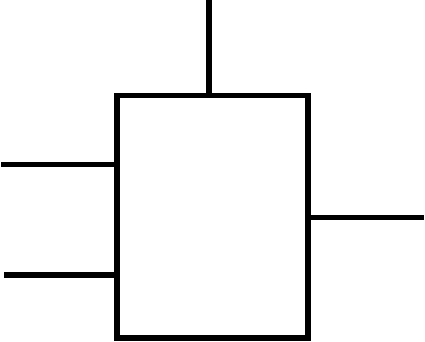
\includegraphics[height=3.5cm,width=4cm]{diagram-20210914(13)-crop}
\end{figure}
Which one of the following is the correct implementation of this multiplexer?
\begin{tasks}(2)
\task[\textbf{A.}] \begin{figure}[H]
	\centering
	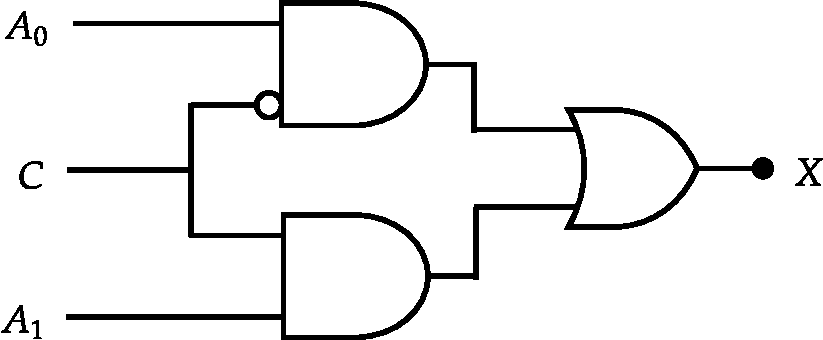
\includegraphics[height=2cm,width=5.5cm]{diagram-20210914(14)-crop}
\end{figure}
\task[\textbf{B.}] \begin{figure}[H]
	\centering
	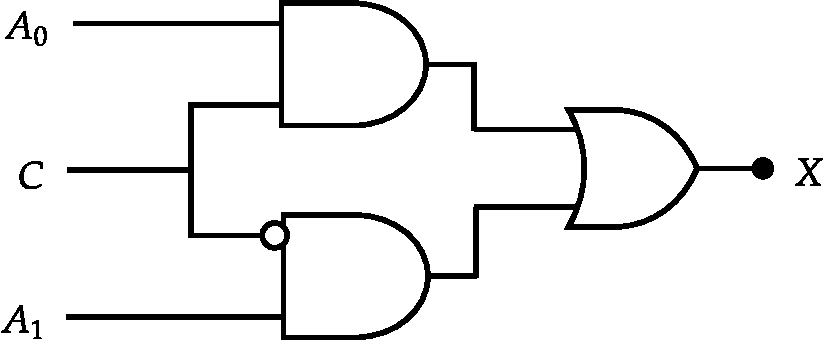
\includegraphics[height=2cm,width=5.5cm]{diagram-20210914(15)-crop}
\end{figure}
\task[\textbf{C.}]\begin{figure}[H]
	\centering
	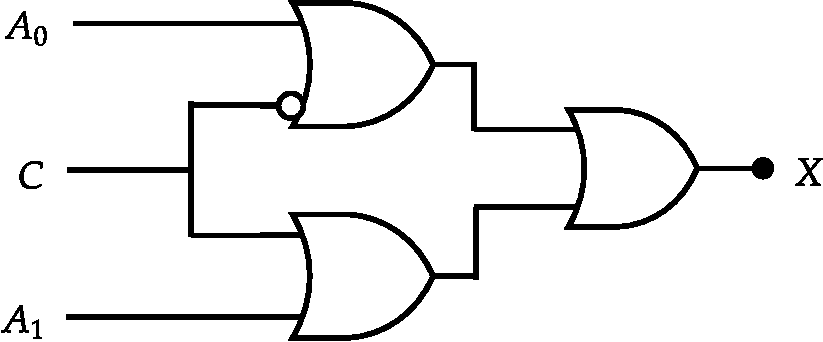
\includegraphics[height=2cm,width=5.5cm]{diagram-20210914(16)-crop}
\end{figure}
\task[\textbf{D.}] \begin{figure}[H]
	\centering
	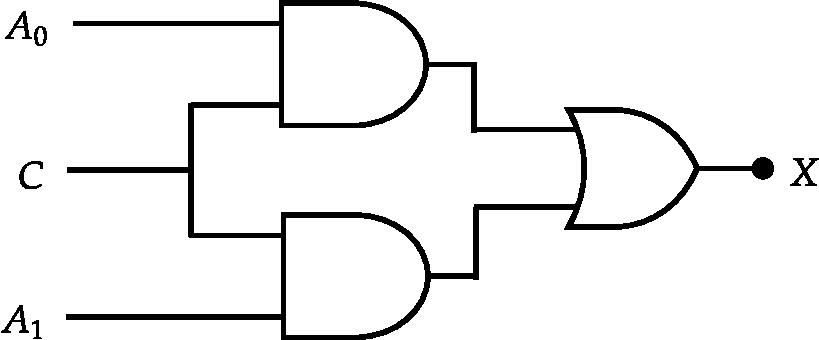
\includegraphics[height=2cm,width=5.5cm]{diagram-20210914(17)-crop}
\end{figure}
\end{tasks}
\begin{answer}
\begin{align*}
\text{Check option (a),}\\
X&=A_{0} \bar{C}+A_{1} C\\
\text{	If }C&=0 \Rightarrow X=A_{0}\\
\text{If }C&=1 \Rightarrow X=A_{1}
\end{align*}
So the correct answer is \textbf{Option (A)}
\end{answer}
	\item Consider the following Boolean expression:
	$$
	(\bar{A}+\bar{B})[\overline{A(B+C)}]+A(\bar{B}+\bar{C})
	$$
	It can be represented by a single three-input logic gate. Identify the gate
\begin{tasks}(4)
\task[\textbf{A.}]  AND
\task[\textbf{B.}] OR
\task[\textbf{C.}] XOR
\task[\textbf{D.}] NAND
\end{tasks}
\begin{answer}
\begin{align*}
Y&=(\bar{A}+\bar{B})[\overline{A(B+C)}]+A(\bar{B}+\bar{C})\\
Y&=(\bar{A}+\bar{B})[\bar{A}+\overline{(B+C)}]+A \bar{B}+A \bar{C}\\
&=(\bar{A}+\bar{B})[\bar{A}+\bar{B} \bar{C}]+A \bar{B}+A \bar{C}\\
&=\bar{A}+\bar{A} \bar{B} \bar{C}+\bar{A} \bar{B}+\bar{B} \bar{C}+A \bar{B}+A \bar{C}\\
&=\bar{A}+\bar{A} \bar{B} \bar{C}+\bar{B} \bar{C}+\bar{A} \bar{B}+A \bar{B}+A \bar{C}\\
&=\bar{A}+\bar{B} \bar{C}+\bar{B}+A \bar{C}=\bar{A}+\bar{B}+A \bar{C}\\
&=(\bar{A}+A \bar{C})+\bar{B}=(A+\bar{A} \bar{C})+\bar{B}=\bar{A}+\bar{C}+\bar{B}\\
Y&=\overline{A B C}
\end{align*}
\end{answer}
	\item The following Boolean expression
	$$
	Y=A \cdot \bar{B} \cdot \bar{C} \cdot \bar{D}+\bar{A} \cdot B \cdot \bar{C} \cdot D+\bar{A} \cdot \bar{B} \cdot \bar{C} \cdot D+\bar{A} \cdot \bar{B} \cdot C \cdot D+\bar{A} \cdot B \cdot C \cdot D+A \cdot \bar{B} \cdot \bar{C} \cdot D \quad \text { can }
	$$
	be simplified to
\begin{tasks}(2)
\task[\textbf{A.}] $\bar{A} \bullet \bar{B} \bullet C+A \bullet \bar{D}$
\task[\textbf{B.}]  $\bar{A} \bullet B \bullet \bar{C}+A \bullet \bar{D}$
\task[\textbf{C.}] $A \bullet \bar{B} \bullet \bar{C}+\bar{A} \bullet D$
\task[\textbf{D.}]  $A \bullet \bar{B} \bullet C+\bar{A} \bullet D$
\end{tasks}
\begin{answer}
\begin{figure}[H]
	\centering
	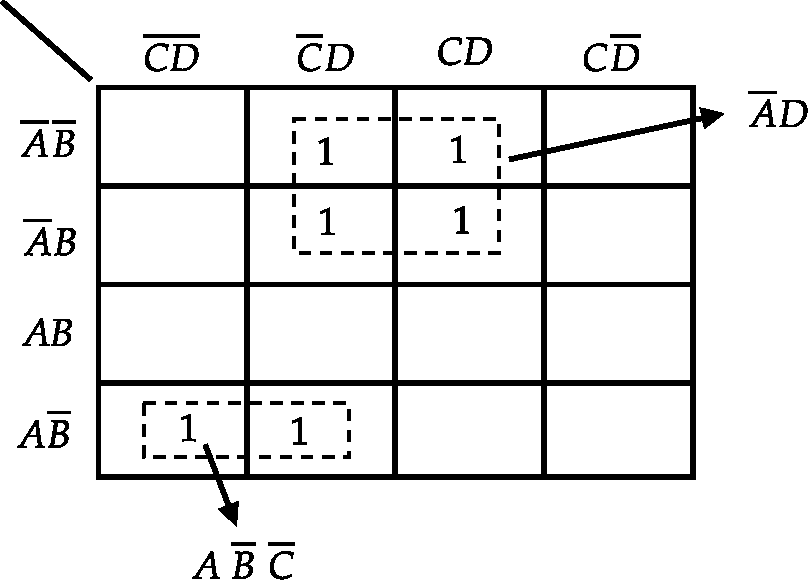
\includegraphics[height=5cm,width=7.5cm]{diagram-20210913(7)-crop}
\end{figure}
So the correct answer is \textbf{Option (C)}
\end{answer}
	\item The voltage resolution of a 12 -bit digital to analog converter (DAC), whose output varies from $-10 V$ to $+10 V$ is, approximately
\begin{tasks}(4)
\task[\textbf{A.}] $1\  \mathrm{mV}$
\task[\textbf{B.}] $5 \ \mathrm{mV}$
\task[\textbf{C.}] $20 \ \mathrm{mV}$
\task[\textbf{D.}] $100 \ \mathrm{mV}$
\end{tasks}
\begin{answer}
\begin{align*}
\text{Voltage resolution }&=\frac{20 \mathrm{~V}}{2^{12}-1}=4.8 \mathrm{mV}
\end{align*}
So the correct answer is \textbf{Option (B)}
\end{answer}
	\item For any set of inputs, A and B, the following circuits give the same output, Q, except one. Which one is it?
\begin{tasks}(2)
\task[\textbf{A.}] \begin{figure}[H]
	\centering
	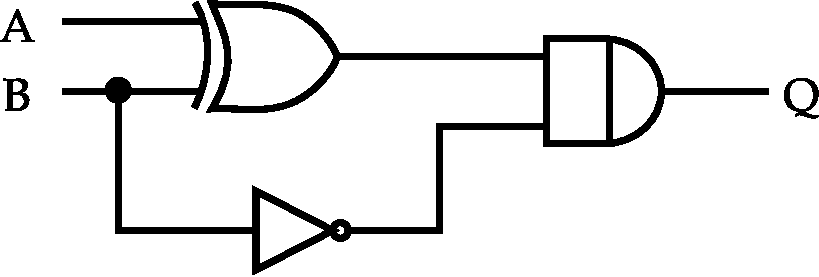
\includegraphics[height=2.5cm,width=7cm]{diagram-20210912(13)-crop}
\end{figure}
\task[\textbf{B.}]\begin{figure}[H]
	\centering
	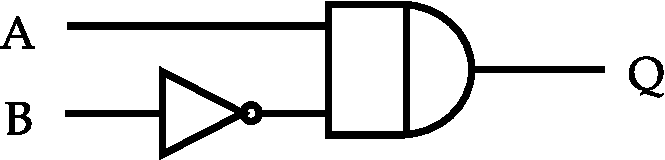
\includegraphics[height=1.5cm,width=6cm]{diagram-20210912(14)-crop}
\end{figure}
\task[\textbf{C.}] \begin{figure}[H]
	\centering
	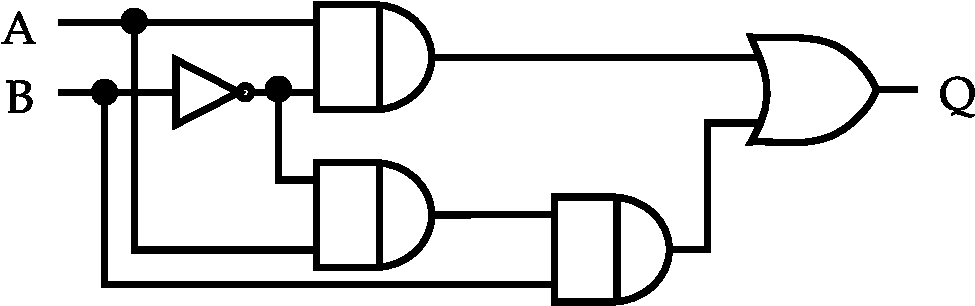
\includegraphics[height=2.5cm,width=7.5cm]{diagram-20210912(15)-crop}
\end{figure}
\task[\textbf{D.}]\begin{figure}[H]
	\centering
	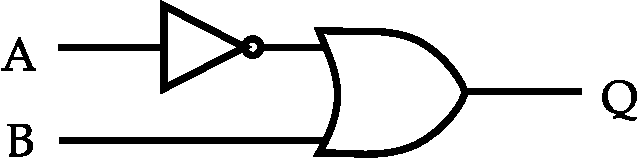
\includegraphics[height=1.5cm,width=6cm]{diagram-20210912(16)-crop}
\end{figure}
\end{tasks}
\begin{answer}
So the correct answer is \textbf{Option (D)}
\end{answer}
	\item A counter consists of four flip-flops connected as shown in the figure:\\
	\begin{figure}[H]
		\centering
		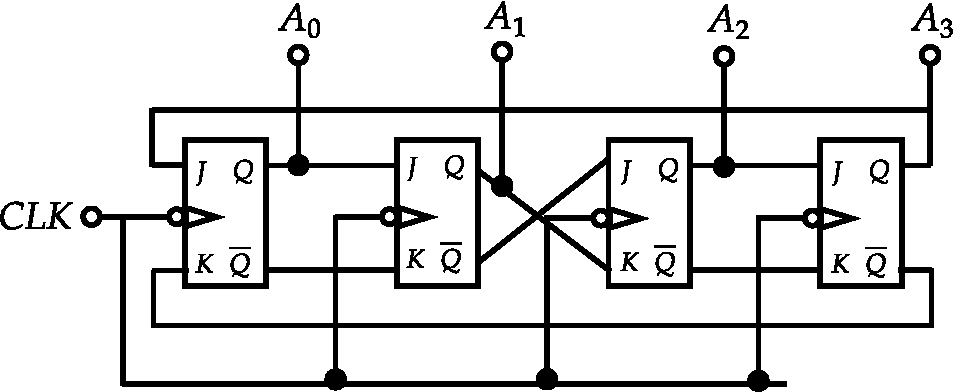
\includegraphics[height=3.5cm,width=7.5cm]{diagram-20211018(3)-crop}
	\end{figure}
	If the counter is initialized as $A_{0} A_{1} A_{2} A_{3}=0110$, the state after the next clock pulse is
\begin{tasks}(4)
\task[\textbf{A.}] 1000
\task[\textbf{B.}] 0001
\task[\textbf{C.}] 0011
\task[\textbf{D.}] 1100
\end{tasks}
\begin{answer}$\left. \right. $
\begin{figure}[H]
	\centering
	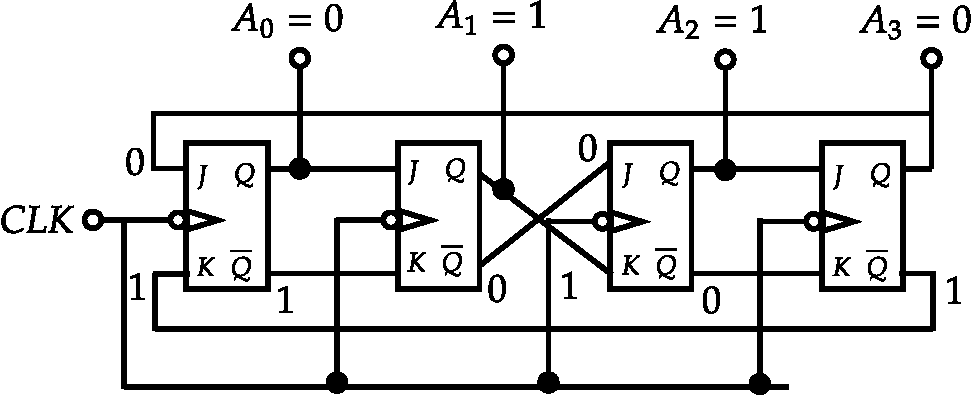
\includegraphics[height=3.5cm,width=7.5cm]{e5s}
\end{figure}
So the correct answer is \textbf{Option (B)}
\end{answer}
	\item The logic circuit shown in the figure below Implements the Boolean expression
\begin{figure}[H]
\centering
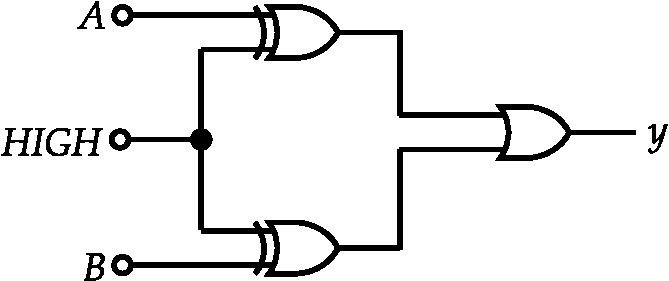
\includegraphics[height=2.5cm,width=6cm]{e-14}
\end{figure}
\begin{tasks}(4)
\task[\textbf{A.}] $y=\overline{A \cdot B}$
\task[\textbf{B.}] $y=\bar{A} \cdot \bar{B}$
\task[\textbf{C.}] $y=A \cdot B$
\task[\textbf{D.}] $y=A+B$
\end{tasks}
\begin{answer}
\begin{align*}
\text{Output of each Ex-OR gate is }\bar{A} and \bar{B}.\text{ Thus }y=\bar{A}+\vec{B}=\overline{A \cdot B}
\end{align*}
So the correct answer is \textbf{Option (A)}
\end{answer}
\item 	If one of the inputs of a J-K flip flop is high and the other is low, then the outputs $Q$ and $\bar{Q}$
\begin{tasks}(1)
\task[\textbf{A.}] Oscillate between low and high in race around condition
\task[\textbf{B.}] Toggle and the circuit acts like a $T$ flip flop
\task[\textbf{C.}] Are opposite to the inputs
\task[\textbf{D.}] Follow the inputs and the circuit acts like an $R-S$ flip flop
\end{tasks}
\begin{answer}
So the correct answer is \textbf{Option (D)}
\end{answer}
	\item The state diagram corresponding to the following circuit is
\begin{figure}[H]
\centering
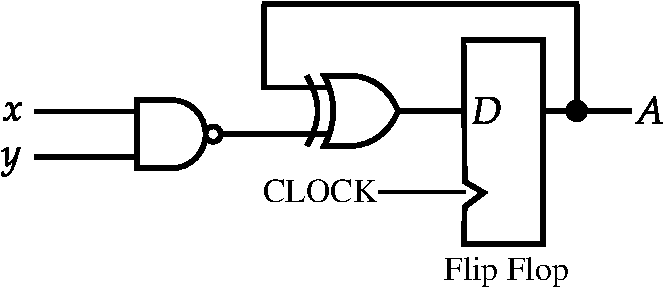
\includegraphics[height=3cm,width=6cm]{e41}
\end{figure}
\begin{tasks}(2)
\task[\textbf{A.}] \begin{figure}[H]
	\centering
	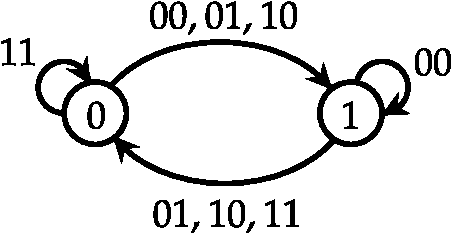
\includegraphics[height=2cm,width=3.8cm]{e41a}
\end{figure}
\task[\textbf{B.}] \begin{figure}[H]
	\centering
	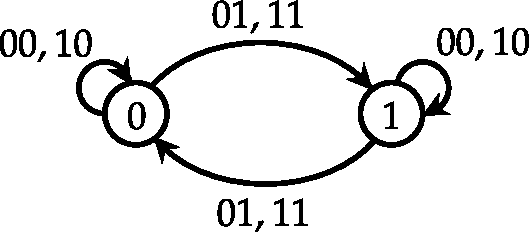
\includegraphics[height=2cm,width=3.8cm]{e41b}
\end{figure}
\task[\textbf{C.}] \begin{figure}[H]
	\centering
	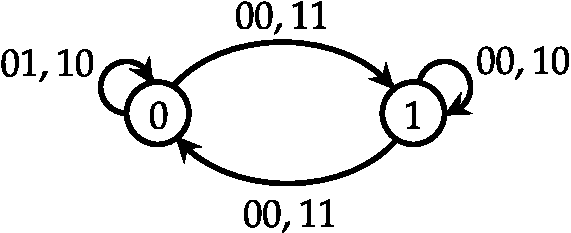
\includegraphics[height=2cm,width=3.8cm]{e41c}
\end{figure}
\task[\textbf{D.}] \begin{figure}[H]
	\centering
	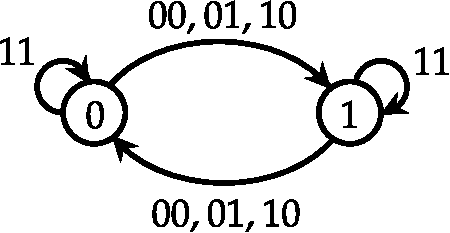
\includegraphics[height=2cm,width=3.8cm]{e41d}
\end{figure}
\end{tasks}
\begin{answer}
\begin{align*}
D_{A}=\overline{x y} \oplus A
\end{align*}
\begin{align*}
\renewcommand*{\arraystretch}{1.5}
\begin{tabular}{|c|c|c|c|}
\hline
Input
$x \quad y$&Present
State A&Flip-Flop
Input $D_{A}$&Next State
$\mathrm{A}$\\
\hline
0 0&0&1&1\\
\hline
0 0&1&0&0\\
\hline
0 1&0&1&1\\
\hline
0 1&1&0&0\\
\hline
1 0&0&1&1\\
\hline
1 0& 1& 0&0\\
\hline
1 1&0&0&0\\
\hline
1 1&1&1&1\\
\hline
\end{tabular}
\end{align*}
So the correct answer is \textbf{Option (D)}
\end{answer}
	\item Which of the following circuits implements the Boolean function
	$$F(A, B, C)=\sum(1,2,4,6) ?$$
\begin{tasks}(2)
\task[\textbf{A.}] \begin{figure}[H]
	\centering
	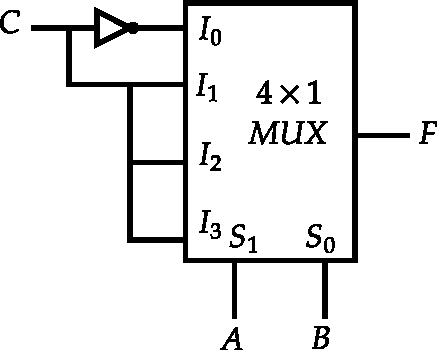
\includegraphics[height=3.5cm,width=4.5cm]{e47a}
\end{figure}
\task[\textbf{B.}] \begin{figure}[H]
	\centering
	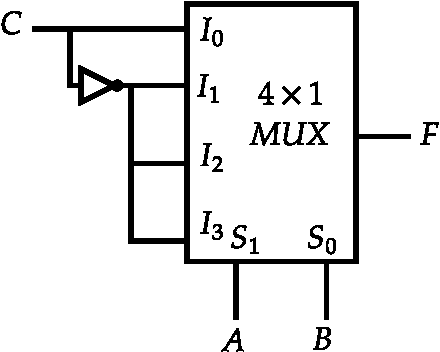
\includegraphics[height=3.5cm,width=4.5cm]{e47b}
\end{figure}
\task[\textbf{C.}] \begin{figure}[H]
	\centering
	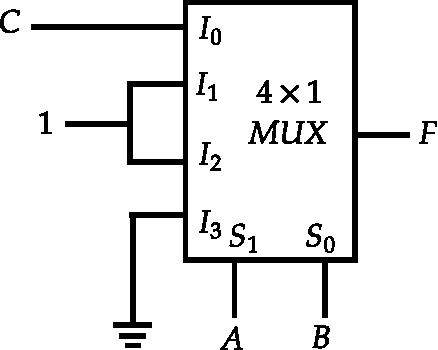
\includegraphics[height=3.5cm,width=4.5cm]{e47c}
\end{figure}
\task[\textbf{D.}] \begin{figure}[H]
	\centering
	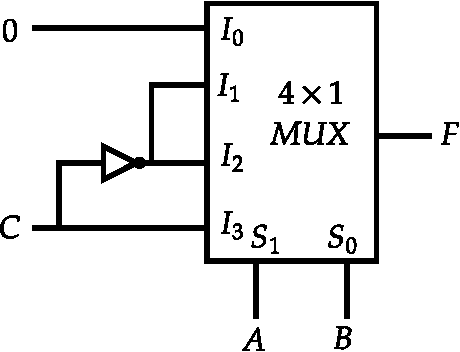
\includegraphics[height=3.5cm,width=4.5cm]{e47d}
\end{figure}
\end{tasks}
\begin{answer}
\begin{align*}
\renewcommand*{\arraystretch}{1}
\begin{tabular}{|p{1.5cm} p{1.5cm} p{1.5cm}|p{1.5cm}p{2cm}|}
\hline
A&B&C&F&$\left. \right. $\\
\hline
0&0&0&0&\\
0&0&1&1&F=C\\\hline
0&1&0&1&\\
0&1&1&0&F=$\bar{C}$\\\hline
1&0&0&1&\\
1&0&1&0&F=$\bar{C}$\\\hline
1&1&0&1&\\
1&1&1&0&F=$\bar{C}$\\\hline
\end{tabular}
\end{align*}
So the correct answer is \textbf{Option (B)}
\end{answer}
	\item The circuit below comprises of $D$-flip flops. The output is taken from $Q_{3}, Q_{2}, Q_{1}$ and $Q_{0}$ as shown in the figure.\\
	\begin{figure}[H]
		\centering
		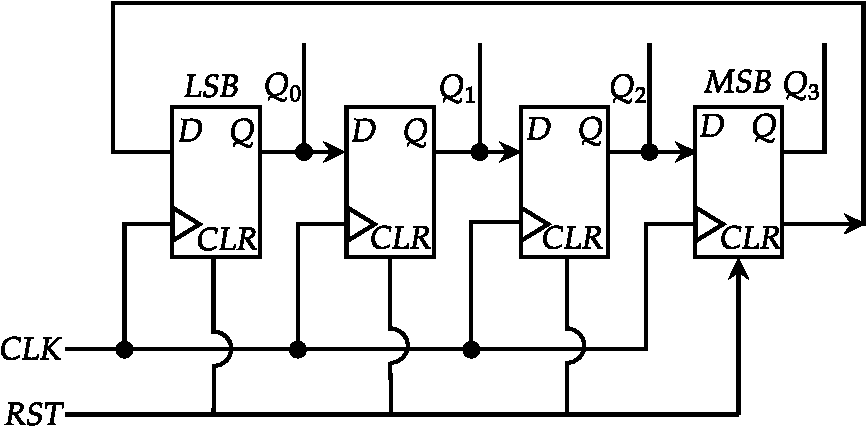
\includegraphics[height=3.5cm,width=7cm]{e66}
	\end{figure}
	the binary number given by the string $Q_{3}, Q_{2}, Q_{1} Q_{0}$ changes for every clock pulse that is applied to the CLK input. If the output is initialized at 0000 , the the corresponding sequence of decimal numbers that repeats itself, is
\begin{tasks}(2)
\task[\textbf{A.}] $3,2,1,0$
\task[\textbf{B.}] $1,3,7,14,12,8$
\task[\textbf{C.}] $1,3,7,15,12,14,0$
\task[\textbf{D.}] $1,3,7,15,14,12,8,0$
\end{tasks}
\begin{answer}
\begin{figure}[H]
	\centering
	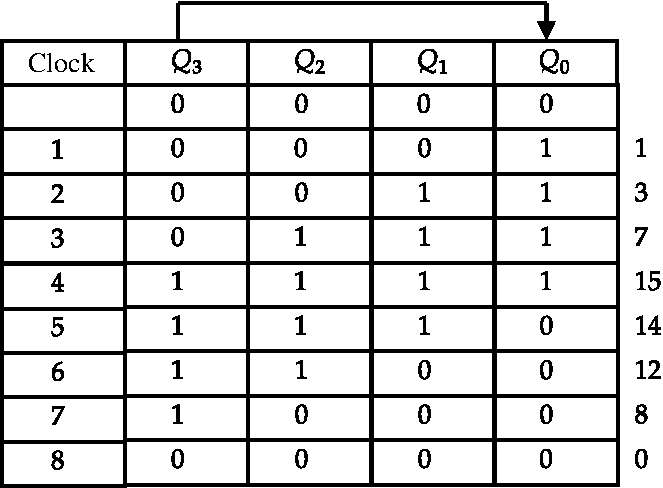
\includegraphics[height=6cm,width=7cm]{e66s}
\end{figure}0
So the correct answer is \textbf{Option (D)}
\end{answer}
	\item In the 3 -bit register shown below, $Q_{1}$ and $Q_{3}$ are the least and the most significant bits of the output, respectively.\\
	\begin{figure}[H]
		\centering
		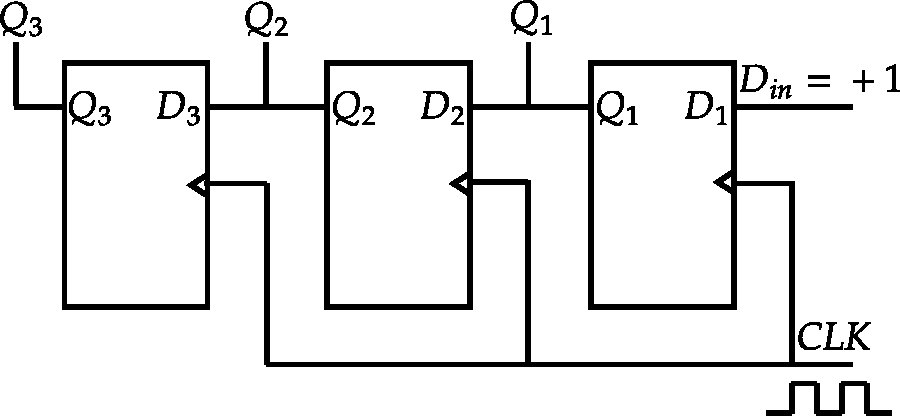
\includegraphics[height=3.5cm,width=8cm]{diagram-20211029(13)-crop}
	\end{figure}
	If $Q_{1}, Q_{2}$ and $Q_{3}$ are set to zero initially, then the output after the arrival of the second falling clock (CLK) edge is
\begin{tasks}(4)
\task[\textbf{A.}]  001
\task[\textbf{B.}] 100
\task[\textbf{C.}]  011
\task[\textbf{D.}]  110
\end{tasks}
\begin{answer}
\begin{align*}
\begin{tabular}{|ccc|c}
\hline
$Q_3$&$Q_3$&$Q_1$&$ $\\
\hline
0&0&1&(1)\\
\hline 
0&1&1&(2)\\
\hline
\end{tabular}
\end{align*}
So the correct answer is \textbf{Option (C)}
\end{answer}
	\item The Boolean equation $Y=\bar{A} B C+\bar{A} B \bar{C}+A \bar{B} \bar{C}+A \bar{B} C$ is to be implemented using only twoinput NAND gates. The minimum number of gates required is
\begin{tasks}(4)
\task[\textbf{A.}] 3
\task[\textbf{B.}] 4
\task[\textbf{C.}] 5
\task[\textbf{D.}] 6
\end{tasks}
\begin{answer}$\left. \right. $
\begin{figure}[H]
	\centering
	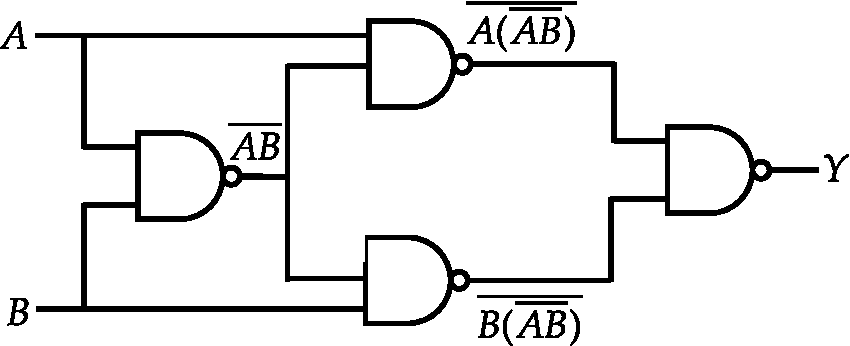
\includegraphics[height=3cm,width=8cm]{diagram-20211029(15)-crop}
\end{figure}
\begin{align*}
Y&=\bar{A} B C+\bar{A} B \bar{C}+A \bar{B} \bar{C}+A \bar{B} C \\ \Rightarrow Y&=\bar{A} B(C+\bar{C})+A \bar{B}(\bar{C}+C)\\
\Rightarrow Y&=\bar{A} B+A \bar{B} \quad(E x-O R)\\
\text{Implementing }&\text{Ex-OR Gate}\\
\Rightarrow Y&=\overline{(A(\overline{A B}))(B(\overline{A B}))}=\overline{A(\overline{A B})}+\overline{B(\overline{A B})} Y\\& =A(\bar{A}+\bar{B})+B(\bar{A}+\bar{B})\\
\text{So minimum 4 number of}&\text{ gates are required.}
\end{align*}
So the correct answer is \textbf{Option (B)}
\end{answer}
	\item What is $Y$ for the circuit shown below?
\begin{figure}[H]
\centering
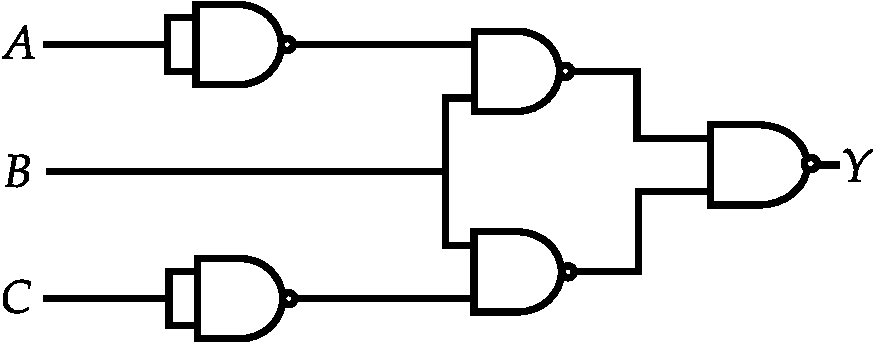
\includegraphics[height=2.5cm,width=7cm]{diagram-20210816(16)-crop}
\end{figure}
\begin{tasks}(2)
\task[\textbf{A.}] $Y=\overline{(A+\bar{B})(\bar{B}+C)}$
\task[\textbf{B.}]  $Y=\overline{(A+\bar{B})(B+C)}$
\task[\textbf{C.}] $Y=\overline{(\bar{A}+B)(\bar{B}+C)}$
\task[\textbf{D.}] $Y=\overline{(A+B)(\bar{B}+C)}$
\end{tasks}
\begin{answer}
\begin{figure}[H]
	\centering
	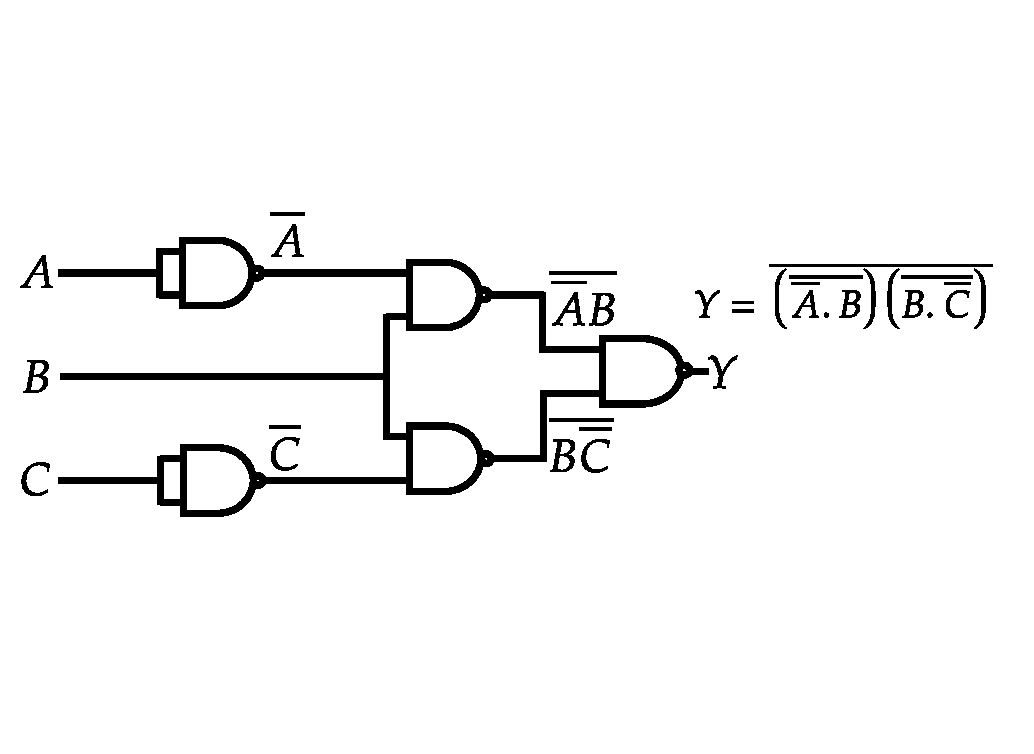
\includegraphics[height=7cm,width=10cm]{diagram-20210816(17)}
\end{figure}
\begin{align*}
Y&=\overline{(\overline{\bar{A}} B) \cdot(\overline{B . \bar{C}})}=\overline{(A+\bar{B})(\bar{B}+C)}
\end{align*}
So the correct answer is \textbf{Option (A)}
\end{answer}
	
	
	
	
	
	
	
	
	
	
	
	
	
	
\end{enumerate}